\section{Experimental setup}
\label{sec:setup}

\begin{figure*}[t]
  \centering
  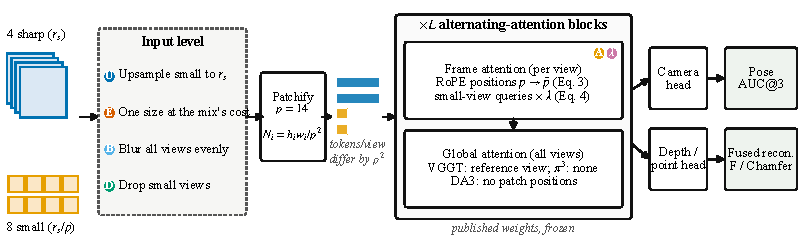
\includegraphics[width=\textwidth]{figures/fig_arch.pdf}
  \caption{\textbf{Where each intervention acts.} The three models share an alternating design: each view is cut into patches, attends within itself (frame attention, with 2D rotary positions), then attends across all views (global attention), and heads predict cameras and depth. In a mixed input, views have different token counts. Input-level interventions (U, E, B, D) change what the model sees. In-model corrections act on frame attention: position alignment (A, \cref{eq:align}) and attention scaling ($\lambda$, \cref{eq:lambda}). The models differ in global attention, which makes \dathree a control for cross-view position effects. Weights stay frozen throughout.}
  \label{fig:arch}
\end{figure*}

\paragraph{Models.}
We use the published weights of VGGT-1B, \pithree and \dathree-Large at pinned code versions, without retraining, in 16-bit floating point. All three use $14{\times}14$ patches. \Cref{tab:models} lists the properties that matter for mixed input. The difference that matters most is in global attention: VGGT and \pithree give each patch its position on its own view's grid, while \dathree gives every patch the same position.

\begin{table}[t]
\centering\small
\setlength{\tabcolsep}{3pt}
\begin{tabular}{@{}lccc@{}}
\toprule
 & VGGT-1B & \pithree & \dathree-L \\
\midrule
Reference view             & first view & none & first view$^*$ \\
Frame-attention positions  & 2D RoPE & 2D RoPE & 2D RoPE \\
Global-attention positions & 2D RoPE & 2D RoPE & shared (none) \\
Default patches $T$        & 1{,}369 & $\approx$1{,}301 & 1{,}296 \\
\bottomrule
\end{tabular}
\caption{\textbf{Model properties relevant to mixed input.} $T$ is the number of patches per view at each model's default input resolution, used in \cref{eq:lambda}. $^*$\dathree chooses its reference view by a configurable strategy; we use the first view.}
\label{tab:models}
\end{table}

\paragraph{Token budget.}
An input of $n$ views, with view $i$ resized to $h_i\times w_i$ pixels, costs
\begin{equation}
  B \;=\; \sum_{i=1}^{n} \frac{h_i\, w_i}{14^2}
  \label{eq:budget}
\end{equation}
patch tokens. Our main budgets are $B{=}4{,}096$ and $8{,}192$, with $2{,}048$ and $16{,}384$ as extensions. A \emph{uniform} input with $n$ views uses the largest resolution at which all $n$ views fit the budget. Tokens are a fair measure of cost here. Timed on one GPU and one scene per dataset, a mix and a uniform input with the same token count differ in run time by $+2\%$ for \pithree, $-2\%$ for VGGT and $+10\%$ for \dathree; some of the timed \dathree mixes include a low-resolution view-selection pass, which adds to their time. Doubling the tokens makes a run 1.5--1.8$\times$ slower, so token counts translate into real cost.

\paragraph{Mixed inputs.}
For the diagnosis, each scene gets 12 views: $n_s{=}4$ sharp views at resolution $\mixsize$ and $n_m{=}8$ small views at $\mixsize/\rho$, with resolution ratio $\rho\in\{2,3\}$. We also test $\rho{=}4$, the splits 2+10 and 6+6, and graded mixes whose 8 small views take four sizes. The lower token level sets $\mixsize$ to the resolution of an 8-view uniform input at 4{,}096 tokens: a long side of 350\,px for 4:3 images and 378\,px for ETH3D, about 470 tokens per sharp view. The higher level uses the 8-view resolution at 8{,}192 tokens: 504\,px and 546\,px, about 1{,}000 tokens per sharp view, which is close to the 518\,px input VGGT uses by default. A seeded shuffle decides which frames are sharp, and all inputs for a scene draw on the same frames.

\paragraph{Interventions.}
Each intervention changes one factor of the mixed input while the frames stay fixed:
\begin{itemize}[nosep,leftmargin=*]
  \item \textbf{As-is}: each view at its own size, with native positions.
  \item \textbf{Aligned}: the small views' rotary positions mapped onto the sharp grid (\cref{eq:align}).
  \item \textbf{+Attention}: aligned, plus an attention correction on the small views (\cref{eq:lambda}).
  \item \textbf{Upsampled}: small views upsampled (bicubic) to the size their image has at $\mixsize$. This adds no information; token count, spacing and positions now match the sharp views.
  \item \textbf{Shrunk}: all 12 views at the small size.
  \item \textbf{One size}: all 12 views at the common resolution $r_{\mathrm{eq}}=\mixsize\sqrt{(n_s+n_m\rho^{-2})/12}$, at which they cost the same as the mix.
  \item \textbf{Blurred}: all 12 views reduced to the small views' resolution and upsampled back, so no view has more detail than the others.
  \item \textbf{Drop}: the 4 sharp views alone.
  \item \textbf{True}: all 12 views at $\mixsize$, the reference.
\end{itemize}
Upsampled against aligned separates representation from information. True against upsampled measures how much real detail the small views lost.

\paragraph{Datasets.}
We use the five datasets of the \dathree benchmark~\cite{lin2025da3}: ETH3D~\cite{schops2017eth3d} (11 scenes), 7-Scenes~\cite{shotton2013scene} (7), ScanNet++~\cite{yeshwanth2023scannetpp} (20), HiRoom (30, of which 19 have at least 12 frames and are used wherever 12 views are needed) and DTU~\cite{jensen2014large} (22). DTU was never used for any configuration choice, so it serves as a held-out test.

\paragraph{Metrics.}
Pose is measured by \auc, the area under the accuracy curve of relative rotation and translation errors up to 3\textdegree, over all pairs of views in the input. On 7-Scenes we use a version that handles the dataset's non-orthonormal ground-truth rotations. Reconstruction fuses predicted depth with predicted cameras, aligns the result to the ground truth with a similarity transform, and reports F-score on the first four datasets and overall Chamfer distance in millimetres on DTU, following the \dathree protocol. All-pair \auc only scores the views an input contains, so inputs with different view counts are scored on different frames. When we compare such inputs, we also score pose on the four sharp frames that every input shares (\emph{common frames}, 6 pairs). We added this control after the first results were read, and say so wherever it is used.

\paragraph{Protocol and statistics.}
Each study had a written protocol that fixed its design, analysis and predictions before any of its jobs ran. Configurations were chosen on a selection seed (42). Every reported number comes from a different seed (1000), which also draws different frames, so no reported number influenced a choice. The core diagnosis was repeated on a third seed (2000) with new frames. Differences are paired by scene and summarised with a 10{,}000-sample bootstrap over scenes. A difference is \emph{significant} when its mean lies more than two standard errors from zero. A \emph{cell} is one model, dataset and setting; we report significant wins and losses over cells as W/L, and the remaining cells are inconclusive. We never pool across budgets, tasks or datasets.
